\chapter{Analysis and Specification of Requirements}
\label{chap:requirements}

The requirement analysis defines the actors, functional, and non-functional
requirements to ensure the system meets user needs and operational goals.
By identifying actors and their roles, we tailor the system to support
effective probabilistic electricity demand forecasting. The system will
deliver the necessary functionality, meet performance metrics and provide an intuitive experience for accurate and timely forecasting decisions.

\section{Requirement Analysis}
\label{sec:req_analysis}

The requirement analysis process identifies who interacts with the system,
what they need it to do, and under what quality constraints it must operate.

\subsection{Actors Identification}
\label{subsec:actors}

The system serves various stakeholders with distinct roles and responsibilities.These actors are categorized into primary and secondary groups based on their interaction frequency and criticality to core system operations.

\subsubsection{Primary Actors}

The following actors interact directly and frequently with the forecasting system:

\begin{enumerate}
    \item \textbf{Energy Grid Operators}: Responsible for real-time grid management and load balancing operations.
    
    \item \textbf{Energy Traders}: Professionals who make trading decisions based on electricity demand forecasts.

\end{enumerate}

\subsubsection{Secondary Actors}

The following actors have less frequent but important interactions with the system:

\begin{enumerate}
    \item \textbf{Energy Planners}: Strategic decision-makers for long-term infrastructure planning.
    \item \textbf{System Administrators}: Technical staff responsible for infrastructure management and system maintenance.
\end{enumerate}

Primary actors interact with the system daily for operational decision-making, while secondary actors use the system periodically for strategic planning and administrative tasks.

\subsection{Functional Requirements}
\label{subsec:func_req}

The functional requirements describe the specific tasks and actions each
actor should be able to perform within the system. These requirements are
outlined as follows:

\begin{table}[H]
\centering
\caption{Actor Functional Needs}
\label{tab:functional_needs}
\begin{tabular}{|p{7cm}|p{9cm}|}
\hline
\textbf{Actor} & \textbf{Functional Needs} \\
\hline
\multicolumn{2}{|c|}{\textbf{PRIMARY ACTORS}} \\
\hline
\textbf{Energy Grid Operators} &
\begin{itemize}[leftmargin=*, nosep, topsep=2pt, partopsep=0pt]
  \item Generate prediction intervals for 48-hour horizon
  \item Trigger alerts when predicted demand exceeds capacity thresholds
  \item Display historical forecasts vs.\ actual consumption
  \item Provide real-time dashboard with automatic updates
\end{itemize} \\
\hline
\textbf{Energy Traders} &
\begin{itemize}[leftmargin=*, nosep, topsep=2pt, partopsep=0pt]
  \item Generate multiple quantile levels for risk assessment
  \item Export forecast data
  \item Allow custom quantile selection
\end{itemize} \\
\hline
\multicolumn{2}{|c|}{\textbf{SECONDARY ACTORS}} \\
\hline
\textbf{Energy Planners} &
\begin{itemize}[leftmargin=*, nosep, topsep=2pt, partopsep=0pt]
  \item Generate long-term forecast scenarios with uncertainty
  \item Access trend analysis and seasonality reports
  \item View strategic planning dashboards
  \item Export planning reports
\end{itemize} \\
\hline
\textbf{System Administrators} &
\begin{itemize}[leftmargin=*, nosep, topsep=2pt, partopsep=0pt]
  \item Manage user accounts and assign roles
  \item Configure system settings
  \item Access audit logs and security events
\end{itemize} \\
\hline
\multicolumn{2}{|c|}{\textbf{COMMON FUNCTIONAL NEEDS (ALL ACTORS)}} \\
\hline
\textbf{All Users} &
\begin{itemize}[leftmargin=*, nosep, topsep=2pt, partopsep=0pt]
  \item Upload and manage multiple time series
  \item Preprocess data automatically (handle missing values, outliers)
  \item Authenticate securely and access role-based features
\end{itemize} \\
\hline
\end{tabular}
\end{table}

\subsection{Non-Functional Needs}
\label{subsec:nonfunc_req}

Beyond functional capabilities, the system must meet critical non-functional requirements to ensure production-grade performance, reliability, and security.
\subsubsection{Scalability Requirements}
The system architecture must accommodate growing data volumes and user concurrency.
\begin{itemize}
    \item Rescaling time series that don’t have the same length or frequency.
    \item Concurrent user support for multiple simultaneous requests.
\end{itemize}

\subsubsection{Reliability Requirements}
The system must maintain high availability and robust error handling mechanisms.
\begin{itemize}  
    \item Fault tolerance with automatic recovery from training failures.
    \item Data integrity with consistent quantile predictions (monotonicity guaranteed).
    \item Error handling with alert trigger.
\end{itemize}

\subsubsection{Security Requirements}
The system must implement comprehensive security measures to protect sensitive energy data and ensure authorized access.
\begin{itemize}
    \item Data protection with encryption of sensitive consumption data.
    \item Access control with role based authentication and authorization.
\end{itemize}

\subsubsection{Reliability}
\begin{itemize}
    \item Quantile forecasts must be monotonically non-decreasing in
          $\tau$ (no quantile crossing), enforced by post-hoc sorting
          before any result is returned to the user.
    \item The system must recover automatically from model inference
          failures via checkpoint resumption.
\end{itemize}

\subsubsection{Conformity}
\begin{itemize}
    \item The system must comply with relevant data privacy regulations
          (GDPR) to ensure confidentiality of commercially sensitive
          electricity demand data, including AES-256 encryption at rest
          and TLS 1.3 in transit.
    \item All data access and configuration changes must be recorded in
          tamper-evident audit logs.
\end{itemize}

\section{Needs of the Domain}
\label{sec:domain_needs}

The domain of probabilistic electricity demand forecasting involves the use
of advanced deep learning models to enhance the accuracy and calibration of
operational forecasts. The key needs of the domain include:

\begin{itemize}
  \item \textbf{Exogenous meteorological drivers:} Temperature is the
        primary determinant of electricity demand, explaining heating and
        cooling loads that can drive demand spikes of 15--20\% above
        seasonal norms during extreme weather events. The system must
        incorporate weather forecast data (temperature, humidity, pressure,
        wind speed) as future-known inputs to accurately forecast these
        demand extremes.

  \item \textbf{Multiple temporal patterns:} European hourly electricity
        demand exhibits strong daily (24-hour), weekly (168-hour), and
        annual seasonality patterns. These patterns must be captured
        faithfully by the forecasting model across the 35 heterogeneous
        EMHIRES countries, whose demand profiles differ substantially in
        shape, amplitude, and temperature sensitivity.

\end{itemize}

\section{Requirements Specification}
\label{sec:req_spec}

To define the functional requirements of our system clearly and unambiguously,
we utilize UML as the primary modeling language to visually represent system
interactions, making it easier to understand how different components work
together and how each actor's needs are addressed.

\subsection{Modeling Language}
\label{subsec:modeling_lang}

Our project adopts UML as the primary modeling language to describe system
functionality and interactions. UML provides a structured approach to system
design through various diagram types such as use case, sequence, activity, package, and class diagrams, ensuring clarity in communication between developers and stakeholders. It helps in capturing user requirements and defining how the system should behave across all interaction scenarios.

\subsection{Use Case Diagram}
\label{subsec:usecase}

The Use Case Diagram represents the interactions between the system and its
users. It highlights the main actors and their associated functionalities,
providing a high-level overview of the system's core operations.  

\begin{figure}[H]
  \centering
  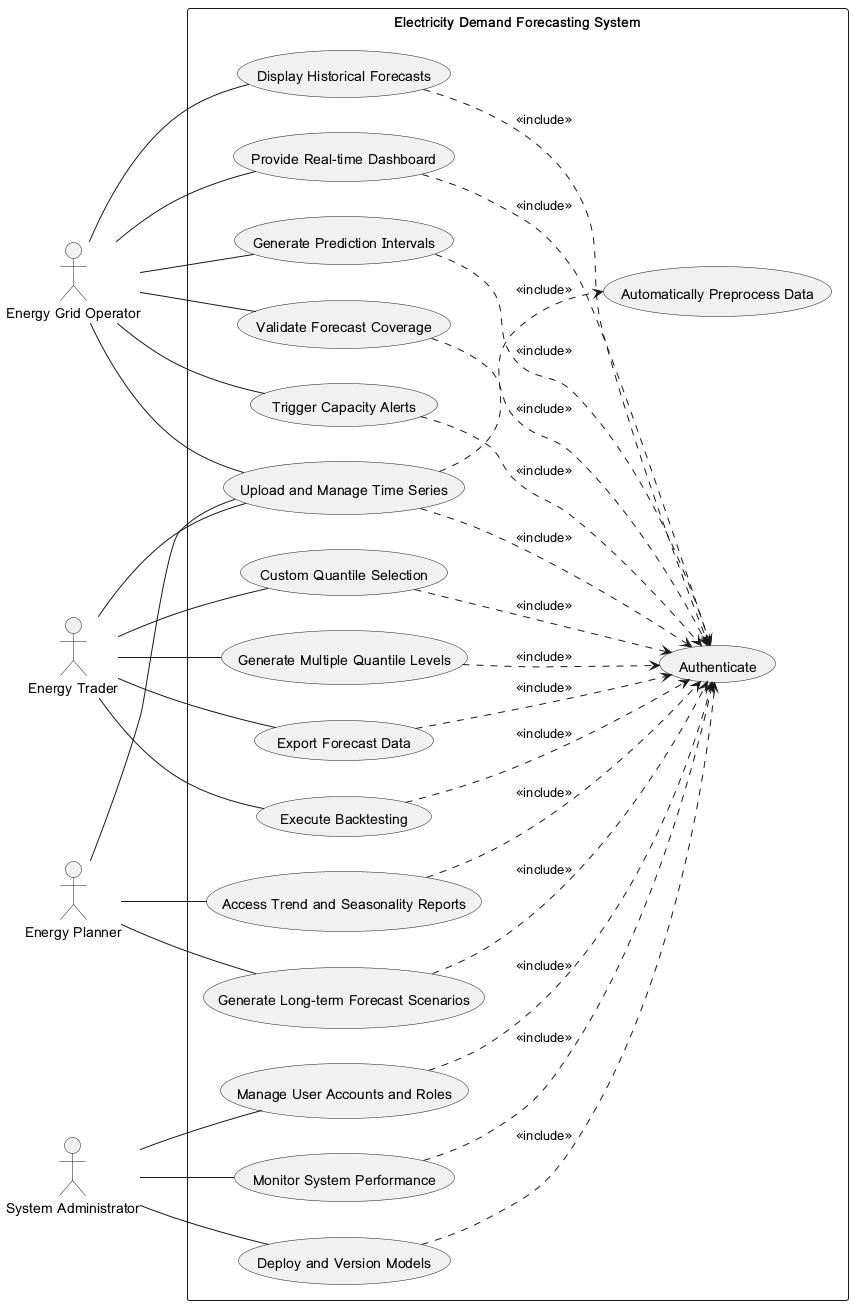
\includegraphics[width=\textwidth,height=0.28\textheight,keepaspectratio]{images/use_case_diagram_en (1).png}
  \caption{Use Case Diagram of the Electricity Demand Forecasting System.}
  \label{fig:usecase}
\end{figure}

\subsection{Sequence Diagrams}
\label{subsec:sequence}

A sequence diagram is a type of UML diagram that illustrates the flow of
messages exchanged during interactions between objects. It presents a set
of elements, represented by lifelines, along with the messages they exchange
throughout their interaction. This particular type of diagram represents
specific execution scenarios of the system.

\begin{figure}[H]
  \centering
  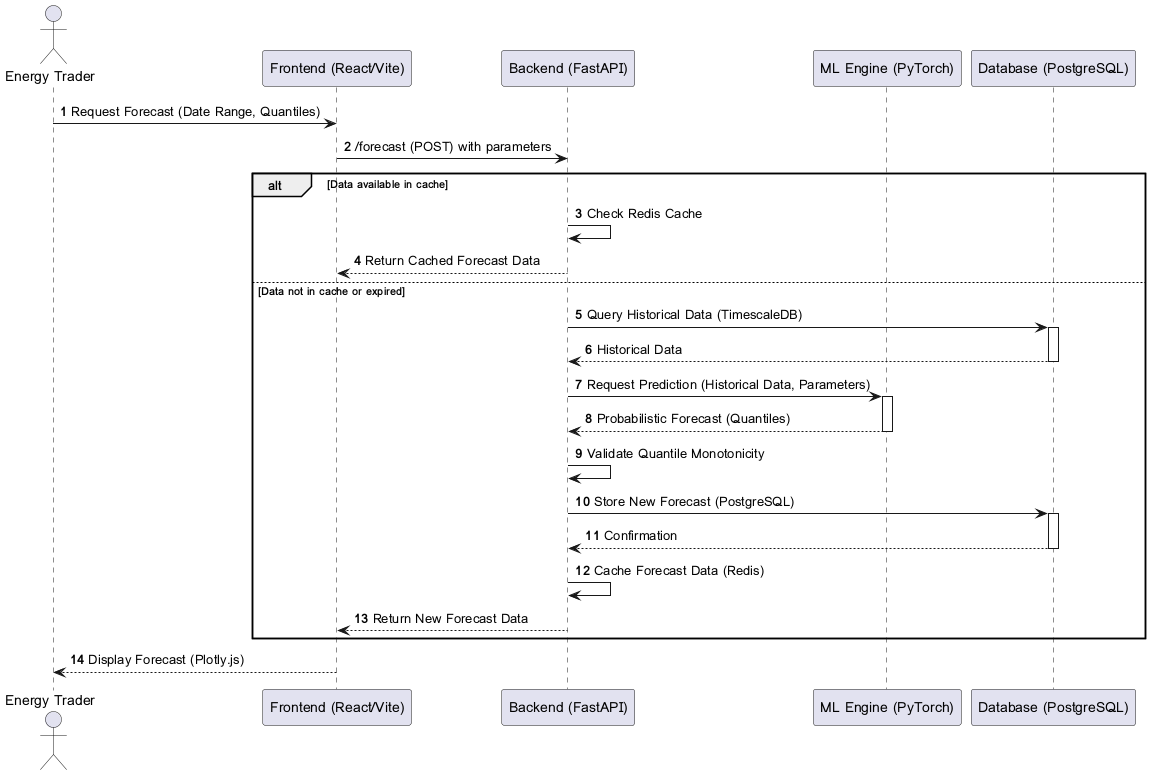
\includegraphics[width=\textwidth]{images/sequence_diagram_en (1).png}
  \caption{Sequence Diagram for the forecast generation use case.}
  \label{fig:seq_requirements}
\end{figure}


